\documentclass[12pt]{ximera}
\title{Final Exam}
\begin{document}
\begin{abstract}
The cumulative final: sets and inclusion-exclusion, the subtraction game, counting
with restrictions, saddle points in zero-sum games, expected value as a decision
tool, and a set of bonus problems drawn from across the semester.
\end{abstract}
\maketitle

\section*{Final Exam}

\begin{problem}
Assess whether each of the following claims is true or false.

\begin{prompt}
\textbf{(a)} Claim: in a \emph{zero-sum} game, every point earned by one of the
players is lost by the other.

\begin{multipleChoice}
\choice[correct]{True}
\choice{False}
\end{multipleChoice}

\begin{feedback}
True --- that is what ``zero-sum'' means. The two players' payoffs always add to
zero, which is why a single payoff matrix from one player's perspective describes the
whole game: Bob's payoff is the negative of the entry shown for Alice.
\end{feedback}
\end{prompt}

\begin{prompt}
\textbf{(b)} Claim: permutations $P(n,k)$ are always \emph{greater than} combinations
$C(n,k)$ for $n$ and $k>1$.

\begin{multipleChoice}
\choice[correct]{True}
\choice{False}
\end{multipleChoice}

\begin{feedback}
True. The two are related by
\[ P(n,k) = C(n,k)\cdot k!, \]
since each unordered selection of $k$ items can be arranged in $k!$ orders. When
$k>1$ we have $k!>1$, so $P(n,k)>C(n,k)$.

(At $k=1$ they are equal, and at $k=0$ both are $1$ --- which is why the claim
restricts to $k>1$.)
\end{feedback}
\end{prompt}
\end{problem}

\begin{problem}
In a survey of $250$ people, $87$ of the participants said they agree that cereal is
a kind of soup (CS), $103$ said they agree that poptarts are a kind of ravioli (PR),
and $58$ said they agree with both.

\begin{prompt}
\textbf{(a)} Fill in all four regions of the Venn diagram.

\begin{center}
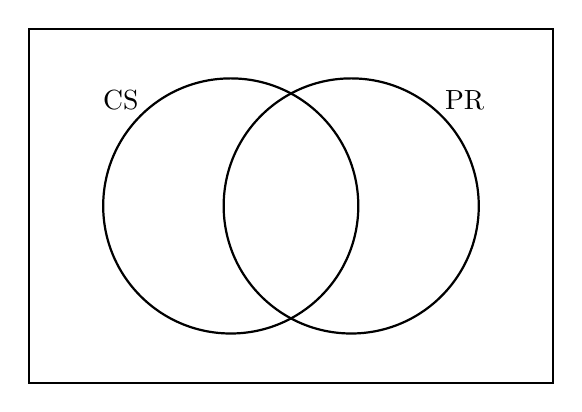
\begin{tikzpicture}[scale=0.9]
  \draw[thick] (-0.85,0) circle (1.8) node at (-2.4,1.5) {CS};
  \draw[thick] (0.85,0) circle (1.8) node at (2.45,1.5) {PR};
  \draw[thick] (-3.7,-2.5) rectangle (3.7,2.5);
\end{tikzpicture}
\end{center}

CS only: $\answer{29}$ \qquad
Both: $\answer{58}$ \qquad
PR only: $\answer{45}$ \qquad
Neither: $\answer{118}$

\begin{hint}
The $87$ and $103$ each already include the $58$ who agreed with both.
\end{hint}

\begin{feedback}
The overlap is $58$. Peeling it off each circle:
\[
\text{CS only} = 87-58 = 29, \qquad \text{PR only} = 103-58 = 45.
\]
Those three regions total $29+58+45=132$, so the region outside both circles is
\[ 250-132 = 118. \]
\end{feedback}
\end{prompt}

\begin{prompt}
\textbf{(b)} What is the (conditional) probability that someone who agrees that cereal
is a kind of soup does NOT agree that poptarts are a kind of ravioli?

Give your answer as a fraction in lowest terms: $\answer{1/3}$

\begin{feedback}
Restrict to the $87$ people who agree cereal is soup. Of those, $29$ are in the ``CS
only'' region, meaning they do not agree about poptarts. So
\[
P\!\left(\olsi{PR}\mid CS\right)=\frac{29}{87}=\frac13.
\]
\end{feedback}
\end{prompt}
\end{problem}

\begin{problem}
Alice and Bob are playing a variation of the Subtraction Game with the following
rules:
\begin{itemize}
\item start with $18$ stones in the pile;
\item on each turn, a player can take $1$, $2$, or $3$ stones;
\item the winner is the player who takes the final stone.
\end{itemize}

\begin{prompt}
If Alice goes first, which player has a winning strategy?

\begin{multipleChoice}
\choice[correct]{Alice, the first player}
\choice{Bob, the second player}
\choice{Neither --- it depends on how Bob plays}
\end{multipleChoice}

\begin{hint}
Work backwards. Which pile sizes are losing positions for the player whose turn it
is? Start with $4$.
\end{hint}

\begin{feedback}
Alice has the winning strategy.

The losing positions --- the pile sizes you do \emph{not} want to face on your turn ---
are the multiples of $4$. If you face $4$ stones, whatever you take ($1$, $2$, or
$3$), your opponent can take the rest and win. If you face $8$, any move leaves
between $5$ and $7$, from which your opponent can move back down to exactly $4$, and
so on.

Since $18$ is not a multiple of $4$ ($18 = 4\cdot 4 + 2$), the first player wins.
\end{feedback}
\end{prompt}

\begin{prompt}
What is that winning strategy? How many stones should Alice take on her first turn?

$\answer{2}$ stones.

\begin{feedback}
Alice takes $2$ stones, leaving $16$ --- a multiple of $4$ --- for Bob.

From then on, she answers each of Bob's moves so that the two moves together remove
exactly $4$ stones: if Bob takes $1$, she takes $3$; if Bob takes $2$, she takes $2$;
if Bob takes $3$, she takes $1$. Each round drops the pile by $4$, so Bob faces
$16, 12, 8, 4$ in turn, and finally $0$ --- meaning Alice took the last stone.
\end{feedback}
\end{prompt}
\end{problem}

\begin{problem}
It's nearly girl scout cookie season, and an office manager needs to choose which six
of the eleven varieties of girl scout cookies currently available to buy for the office.

\begin{prompt}
\textbf{(a)} How many different sets of six could possibly be selected from among the
eleven available cookie varieties?

$\answer{462}$

\begin{feedback}
\[ C(11,6)=\frac{11!}{6!\,5!}=462. \]
\end{feedback}
\end{prompt}

\begin{prompt}
\textbf{(b)} Two of the eleven available varieties are gluten-free. If the manager
wants \emph{exactly one} of the chosen cookie varieties to be gluten-free, how many
different sets of six are possible?

$\answer{252}$

\begin{hint}
Split the decision in two: which gluten-free variety, and which of the others fill
the remaining five slots.
\end{hint}

\begin{feedback}
Choose $1$ of the $2$ gluten-free varieties, and then $5$ of the $9$ remaining
varieties:
\[
C(2,1)\cdot C(9,5) = 2\cdot 126 = 252.
\]
\end{feedback}
\end{prompt}

\begin{prompt}
\textbf{(c)} How many different sets of six don't include \emph{any} gluten-free
varieties?

$\answer{84}$

\begin{feedback}
All six must come from the $9$ varieties that are not gluten-free:
\[ C(9,6)=\frac{9!}{6!\,3!}=84. \]
\end{feedback}
\end{prompt}

\begin{prompt}
\textbf{(d)} If the manager chooses six at random from among the eleven available cookie
varieties, what is the probability that \emph{at least one} of the varieties I select
is gluten-free?

Give your answer as a fraction in lowest terms: $\answer{9/11}$

\begin{feedback}
Use the complement with part (c):
\[
P(\text{no gluten-free}) = \frac{84}{462} = \frac{2}{11},
\]
so
\[
P(\text{at least one}) = 1-\frac{2}{11} = \frac{9}{11}\approx 0.818,
\]
about $81.8\%$.
\end{feedback}
\end{prompt}
\end{problem}

\begin{problem}
The following payoff matrices each represent Alice's perspective for a zero-sum game.
For each one, identify the saddle point if it exists.

Recall the method: find the minimum of each row (the worst Alice can do with that
choice) and take the largest of those; then find the maximum of each column and take
the smallest of those. If the two agree, that value is the saddle point.

\begin{prompt}
\textbf{(a)}
\[
\begin{array}{c|c|c|}
\phantom{|} & c & d \\\hline
a & -3 & 1 \\\hline
b & 0 & 2 \\\hline
\end{array}
\]

Does a saddle point exist?
\begin{multipleChoice}
\choice[correct]{Yes}
\choice{No}
\end{multipleChoice}

If so, its value is $\answer{0}$.

\begin{feedback}
Row minima: row $a$ gives $-3$, row $b$ gives $0$; the largest is $0$.
Column maxima: column $c$ gives $0$, column $d$ gives $2$; the smallest is $0$.

They agree, so there is a saddle point of value $0$, at the entry $(b,c)$.
\end{feedback}
\end{prompt}

\begin{prompt}
\textbf{(b)}
\[
\begin{array}{c|c|c|}
\phantom{|} & c & d \\\hline
a & 4 & -3 \\\hline
b & -1 & 1 \\\hline
\end{array}
\]

Does a saddle point exist?
\begin{multipleChoice}
\choice{Yes}
\choice[correct]{No}
\end{multipleChoice}

\begin{feedback}
Row minima: $-3$ and $-1$; the largest is $-1$.
Column maxima: $4$ and $1$; the smallest is $1$.

Since $-1\neq 1$, there is no saddle point --- this game has no stable pair of pure
strategies, and both players do better mixing.
\end{feedback}
\end{prompt}

\begin{prompt}
\textbf{(c)}
\[
\begin{array}{c|c|c|c|}
\phantom{|} & d & e & f \\\hline
a & -1 & 5 & 0 \\\hline
b & -2 & 0 & -3 \\\hline
c & 2 & 3 & 1 \\\hline
\end{array}
\]

Does a saddle point exist?
\begin{multipleChoice}
\choice[correct]{Yes}
\choice{No}
\end{multipleChoice}

If so, its value is $\answer{1}$.

\begin{feedback}
Row minima: $-1$, $-3$, and $1$; the largest is $1$.
Column maxima: $2$, $5$, and $1$; the smallest is $1$.

They agree, so the saddle point has value $1$, at the entry $(c,f)$.
\end{feedback}
\end{prompt}

\begin{prompt}
\textbf{(d)}
\[
\begin{array}{c|c|c|}
\phantom{|} & d & e \\\hline
a & 0 & -1 \\\hline
b & 1 & 2 \\\hline
c & -2 & 0 \\\hline
\end{array}
\]

Does a saddle point exist?
\begin{multipleChoice}
\choice[correct]{Yes}
\choice{No}
\end{multipleChoice}

If so, its value is $\answer{1}$.

\begin{feedback}
Row minima: $-1$, $1$, and $-2$; the largest is $1$.
Column maxima: $1$ and $2$; the smallest is $1$.

They agree, so the saddle point has value $1$, at the entry $(b,d)$.
\end{feedback}
\end{prompt}
\end{problem}

\begin{problem}
Use your knowledge of game theory and expected values to answer the following.

\begin{prompt}
\textbf{(a)} Complete the payoff matrix from Alice's perspective for a two-player
zero-sum game similar to Rock/Paper/Scissors, except that only Alice has paper and
only Bob has scissors. On the count of three they each signal their choice, with the
understanding that:
\begin{itemize}
\item rock wins \emph{1 point} versus scissors;
\item scissors wins \emph{2 points} versus paper;
\item paper wins \emph{1 point} versus rock.
\end{itemize}

\[
\begin{array}{c|c|c|}
\phantom{|} & \text{Bob: rock} & \text{Bob: scissors} \\\hline
\text{Alice: rock} & \answer{0} & \answer{1} \\\hline
\text{Alice: paper} & \answer{1} & \answer{-2} \\\hline
\end{array}
\]

\begin{hint}
Entries are from Alice's perspective, so a win for Alice is positive and a win for
Bob is negative. Rock against rock is a tie.
\end{hint}

\begin{feedback}
Taking each cell in turn, from Alice's perspective:
\begin{itemize}
\item rock vs.\ rock: a tie, worth $0$.
\item rock vs.\ scissors: rock beats scissors for $1$ point, so $+1$ for Alice.
\item paper vs.\ rock: paper beats rock for $1$ point, so $+1$ for Alice.
\item paper vs.\ scissors: scissors beats paper for $2$ points --- a win for Bob, so
      $-2$ for Alice.
\end{itemize}
\end{feedback}
\end{prompt}

\begin{prompt}
\textbf{(b)} Alice is deciding whether to pack a jacket on her day trip. According to
the weather forecast, there is a $40\%$ chance of clear weather, a $45\%$ chance of
rain without high winds, and a $15\%$ chance of rain plus high winds. Alice has rated
her potential satisfaction in the payoff matrix below.

\[
\begin{array}{c|c|c|c|}
\phantom{|} & \text{clear} & \text{just rain} & \text{rain}+\text{wind} \\\hline
\text{pack a jacket} & -3 & 6 & 10 \\\hline
\text{don't pack a jacket} & 10 & -4 & -10 \\\hline
\end{array}
\]

Expected value of packing a jacket: $\answer[tolerance=0.005]{3}$

\smallskip
Expected value of not packing a jacket: $\answer[tolerance=0.005]{0.7}$

\smallskip
Which should she choose?
\begin{multipleChoice}
\choice[correct]{Pack a jacket}
\choice{Don't pack a jacket}
\end{multipleChoice}

\begin{feedback}
Weight each outcome by the probability of the weather it corresponds to:
\begin{align*}
E(\text{pack}) &= 0.40(-3) + 0.45(6) + 0.15(10)\\
&= -1.2 + 2.7 + 1.5 = 3.0,\\[4pt]
E(\text{don't pack}) &= 0.40(10) + 0.45(-4) + 0.15(-10)\\
&= 4.0 - 1.8 - 1.5 = 0.7.
\end{align*}
Since $3.0 > 0.7$, Alice should pack a jacket.

Note that the single most likely weather outcome does not decide this on its own ---
it is the combination of probability and payoff that matters, and the jacket protects
against the two rainy outcomes that together carry $60\%$ of the probability.
\end{feedback}
\end{prompt}

\begin{prompt}
\textbf{(c)} Alice and Bob are playing a game where on the count of three they each
show a card: either a King or an Ace. Alice's payoff matrix is shown below.

\[
\begin{array}{c|c|c|}
\phantom{|} & \text{Bob: King} & \text{Bob: Ace} \\\hline
\text{Alice: King} & 10 & -20 \\\hline
\text{Alice: Ace} & -10 & 15 \\\hline
\end{array}
\]

What is the expected value of this game overall if Alice plays her King $45\%$ of the
time and her Ace the other $55\%$, and Bob independently plays his King $65\%$ of the
time and his Ace $35\%$?

$\answer[tolerance=0.0005]{-0.9125}$

\begin{hint}
Because the two players choose independently, the probability of landing in a given
cell is the product of the two players' probabilities. Compute all four cell
probabilities, then take the weighted average of the payoffs.
\end{hint}

\begin{feedback}
The four cell probabilities are products, since the choices are independent:
\[
\begin{array}{ll}
P(\text{K},\text{K})=(0.45)(0.65)=0.2925 & P(\text{K},\text{A})=(0.45)(0.35)=0.1575\\
P(\text{A},\text{K})=(0.55)(0.65)=0.3575 & P(\text{A},\text{A})=(0.55)(0.35)=0.1925
\end{array}
\]
(These total $1$. \checkmark) Then
\begin{align*}
E &= 0.2925(10) + 0.1575(-20) + 0.3575(-10) + 0.1925(15)\\
  &= 2.925 - 3.150 - 3.575 + 2.8875\\
  &= -0.9125.
\end{align*}
So with these mixes the game slightly favors Bob: Alice loses about $0.91$ points per
play on average.
\end{feedback}
\end{prompt}
\end{problem}

\begin{problem}
The following are bonus problems from throughout the semester.

\begin{prompt}
\textbf{(a)} Use the Principle of Inclusion-Exclusion to calculate $n(A\cap B)$ if
you know that $n(A)=25$, $n(B)=55$, and $n(A\cup B)=65$.

$\answer{15}$

\begin{feedback}
\[ 65 = 25 + 55 - n(A\cap B) = 80 - n(A\cap B), \]
so $n(A\cap B)=80-65=15$.
\end{feedback}
\end{prompt}

\begin{prompt}
\textbf{(b)} Shade the regions of a three-circle Venn diagram to show $A\cup B$, and
then to show $(A\cup B)\cap C$. Sketch both on paper, then check the solution.

\begin{freeResponse}
\end{freeResponse}

\begin{feedback}
For $A\cup B$, shade both circles entirely --- including the parts that dip into $C$,
since $C$ plays no role in this set.

For $(A\cup B)\cap C$, keep only the part of that shading which also lies inside $C$.
\begin{center}
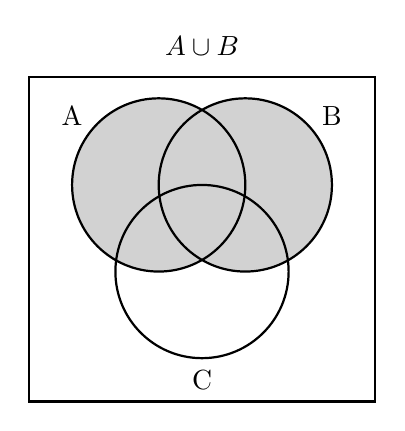
\begin{tikzpicture}[scale=1.1]
  \fill[gray!35] (0,0) circle (1);
  \fill[gray!35] (1,0) circle (1);
  \draw[thick] (0,0) circle (1) node at (-1,0.8) {A};
  \draw[thick] (1,0) circle (1) node at (2,0.8) {B};
  \draw[thick] (0.5,-1) circle (1) node at (0.5,-2.25) {C};
  \draw[thick] (-1.5,-2.5) rectangle (2.5,1.25);
  \node at (0.5,1.6) {$A\cup B$};
\end{tikzpicture}
\qquad
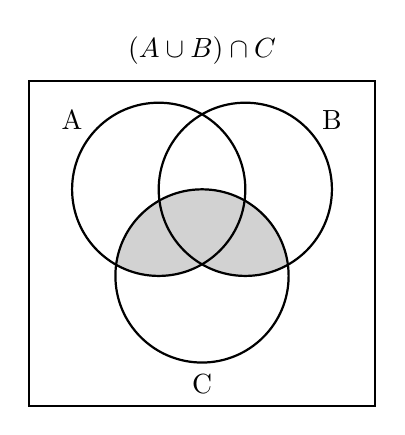
\begin{tikzpicture}[scale=1.1]
  \begin{scope}
    \clip (0.5,-1) circle (1);
    \fill[gray!35] (0,0) circle (1);
    \fill[gray!35] (1,0) circle (1);
  \end{scope}
  \draw[thick] (0,0) circle (1) node at (-1,0.8) {A};
  \draw[thick] (1,0) circle (1) node at (2,0.8) {B};
  \draw[thick] (0.5,-1) circle (1) node at (0.5,-2.25) {C};
  \draw[thick] (-1.5,-2.5) rectangle (2.5,1.25);
  \node at (0.5,1.6) {$(A\cup B)\cap C$};
\end{tikzpicture}
\end{center}
\end{feedback}
\end{prompt}

\begin{prompt}
\textbf{(c)} Calculate by hand the combination $C(10,6)$.

$\answer{210}$

\begin{feedback}
\[
C(10,6)=\frac{10!}{6!\,4!}
=\frac{10\cdot 9\cdot 8\cdot 7}{4\cdot 3\cdot 2\cdot 1}
=\frac{5040}{24}=210.
\]
Note that $C(10,6)=C(10,4)$, so it is easier to cancel the larger factorial.
\end{feedback}
\end{prompt}

\begin{prompt}
\textbf{(d)} Suppose you repeat an experiment five times, and each time the
probability of success is $60\%$. Calculate the (binomial) probability that you record
exactly three successes.

As a percentage rounded to two decimal places: $\answer[tolerance=0.005]{34.56}\%$

\begin{feedback}
\[
P(X=3)=C(5,3)(0.6)^3(0.4)^2 = 10(0.216)(0.16) = 0.3456,
\]
that is, $34.56\%$.
\end{feedback}
\end{prompt}

\begin{prompt}
\textbf{(e)} Calculate the expected winnings of a raffle with the following
probability distribution:

\begin{center}
\begin{tabular}{|r|c|c|c|c|}\hline
Total winnings: & $-\$1$ & \$0 & \$5 & \$10 \\\hline
Probability of each: & $0.6$ & $0.25$ & $0.1$ & $0.05$ \\\hline
\end{tabular}
\end{center}

$\$\answer[tolerance=0.005]{0.40}$

\begin{feedback}
\begin{align*}
E(X) &= 0.6(-1) + 0.25(0) + 0.1(5) + 0.05(10)\\
     &= -0.60 + 0 + 0.50 + 0.50 = 0.40.
\end{align*}
So the expected winnings are $\$0.40$ per raffle --- a favorable game for the player,
even though the most likely single outcome is losing a dollar.
\end{feedback}
\end{prompt}
\end{problem}

\end{document}
